% !TEX root = main.tex
\documentclass[a4paper,12pt]{article}

\usepackage[english, russian]{babel}
\usepackage[T2A]{fontenc}
\usepackage[utf8]{inputenc}

\usepackage{graphicx}
\usepackage{array}
\usepackage{ragged2e}
\usepackage{geometry}
\usepackage{setspace}
\usepackage[style=iso]{datetime2}
\usepackage{amsmath}
\usepackage{amssymb}
\usepackage{amsthm}
\usepackage{enumitem}
\usepackage{multirow}
\usepackage{float}
\usepackage[colorlinks=true, linkcolor=black, urlcolor=blue, pdfborderstyle={/S/U/W 1}]{hyperref}
\usepackage{booktabs}
\usepackage{xcolor}
\usepackage{ulem}
\usepackage{fancyhdr}
\usepackage{lastpage}
\usepackage{indentfirst}
\usepackage{caption}

% Настройка полей
\geometry{top=2cm,bottom=2cm,left=3cm,right=1.5cm}

\pagestyle{fancy}
\fancyhf{}
\renewcommand{\headrulewidth}{0pt}
\cfoot{\thepage}

\usepackage{listings}
\definecolor{codegreen}{rgb}{0,0.6,0}
\definecolor{codegray}{rgb}{0.5,0.5,0.5}
\definecolor{codepurple}{rgb}{0.58,0,0.82}
\definecolor{backcolour}{rgb}{0.95,0.95,0.92}

\lstdefinestyle{mystyle}{
    backgroundcolor=\color{backcolour},   
    commentstyle=\color{codegreen},
    keywordstyle=\color{magenta},
    numberstyle=\tiny\color{codegray},
    stringstyle=\color{codepurple},
    basicstyle=\ttfamily\footnotesize,
    breakatwhitespace=false,         
    breaklines=true,                 
    numbers=left,                    
    numbersep=5pt,                  
    showspaces=false,                
    showstringspaces=false,
    tabsize=2
}

\newtheorem{solution}{Решение}

\begin{document}

    \begin{center}
        \thispagestyle{empty}
        
        % Шапка документа с логотипом
        \begin{minipage}[t]{0.19\textwidth}
            \vspace{-15pt}
            
\includegraphics[width=\linewidth]{logo.png}
        \end{minipage}
        \hfill
        \begin{minipage}[t]{0.8\textwidth}
            \centering
            \scriptsize
            \linespread{1.5}\selectfont
            \textbf{Министерство науки и высшего образования Российской Федерации \\
            Федеральное государственное автономное образовательное учреждение \\
            высшего образования \\
            «Московский государственный технический университет \\
            им. Н.Э. Баумана \\
            (национальный исследовательский университет)» \\
            \vspace{2pt}
            (МГТУ им.\,Н.Э.\,Баумана)}
        \end{minipage}

        \vspace{0.4cm}
        {\rule{\textwidth}{1.2pt}}
        
        % Основная информация
        \vspace{1cm}
        \begin{flushleft}
        \large
        ФАКУЛЬТЕТ: \textbf{ИНФОРМАТИКА И СИСТЕМЫ УПРАВЛЕНИЯ} \\
        \vspace{0.25cm}
        КАФЕДРА: \textbf{КОМПЬЮТЕРНЫЕ СИСТЕМЫ И СЕТИ(ИУ6)} \\
        \vspace{0.25cm}
        НАПРАВЛЕНИЕ: \textbf{09.03.01 Информатика и вычислительная техника}
        \end{flushleft}

        \vspace{1.8cm}
        {\LARGE\bfseries 
        Лабораторная работа №1\\[6pt]
        
        Структуры и методы обработки данных
        }
        
        \vspace{2cm}
        {
        \vspace{0.5cm}
        {\large
        \textbf{Дисциплина:} \underline{Технология разработки программных систем}}

        \vspace{0.5cm}
        \textbf{Вариант:} \underline{№11}
        % Таблица с подписями

        \vspace{3cm}
        \begin{tabular}{lc@{\hspace{8mm}}ccl}
        \textbf{Студент} & \underline{\phantom{1}ИУ6-45Б\phantom{1}} & & \underline{
\includegraphics[width=0.9cm]{signature} 17 февраля}  & \underline{Н.В. Ионов\phantom{1234}}\\
                        & (группа) &  & (Подпись, дата) & (И.О. Фамилия) \\[2.25ex]
                        
        \textbf{Преподаватель} & &  & \underline{\phantom{Подпись, дата}} & \underline{Е.К. Пугачёв\phantom{123}} \\
                            & &  & (Подпись, дата) & (И.О. Фамилия) \\
        \end{tabular}

        \vfill
        {\rule{\textwidth}{0.6pt}}
        \vspace{4pt}
        Москва, 2026
        }
    \end{center}
    \clearpage
    
    \section*{Введение}

    \underline{\textbf{Цель лабораторной работы:}} исследование структур данных, методов их обработки и оценки.
    \vspace{8pt}

    \underline{\textbf{Задание.}}
    \begin{enumerate}
        \item Ознакомиться с теоретическими сведениями об абстрактных структурах данных и методах их обработки. 
        \item Для указанной задачи и структуры данных предложить способ реализации и определить требуемый объем памяти.
        \item Провести анализ заданных  методов поиска, упорядочения  и корректировки  данных.  Оценить  время  выполнения  соответствующих операций. 
        \item Предложить альтернативный вариант решения задачи, в котором должно  быть  минимум одно  улучшение. Улучшения  могут касаться  как  структуры  данных,  так  и  основных  операций.  Обосновать новые решения, используя количественные и качественные критерии.
    \end{enumerate}
    
    \begin{table}[H]
        \centering
        \begin{tabular}{|r|*{4}{c|}}
            \hline
            Задача & Структура данных & Поиск & Упорядовачиние & Корректировка \\
            \hline
            2 & Таблица & Вычисление адреса & Пузырьком & Удаление сдвигом \\
            \hline
        \end{tabular}
        \caption{Условие исходного задания}
    \end{table}

    \underline{\textbf{Задача.}}\vspace{3pt}

    Дана таблица  материальных нормативов, состоящая из $K$ записей фиксированной длины вида: код детали;
    код материала; единица измерения; номер цеха; норма расхода.\vspace{5pt}

    Лабораторная работа будет выполнена на языке \texttt{C}.
    \clearpage

    \section*{Основная часть}
    \refstepcounter{section} 

    \subsection{Реализация}
    Для хранения таблицы будет использоваться статический массив длины $K$.
    Причём элементом этого массива будет запись \texttt{data}.

    \begin{figure}[h]
        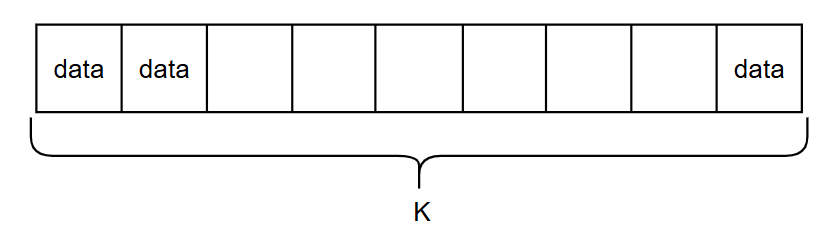
\includegraphics[width=1\textwidth]{vis_const_array}
        \caption{Реализация хранения таблицы в виде статического массива}
    \end{figure}

    Ниже представлен код, который реализует структуру хранения данных.

    \begin{verbatim}
        #define MAX_LEN_UNIT 5
        #define MAX_LEN_MATERIAL 8
        #define MAX_LEN_MEASURE 12 
        #define MAX_LEN_PRODUCTION 8
        #define MAX_LEN_E_CON 4

        typedef struct {
            char unit_code[MAX_LEN_UNIT];
            char material_code[MAX_LEN_MATERIAL];
            char measure[MAX_LEN_MEASURE];
            char production_id[MAX_LEN_PRODUCTION];
            char expected_consumption[MAX_LEN_E_CON];
        } data;

        data table[k];
    \end{verbatim}
    \begin{center}
        \captionof{figure}{Реализации структуры \texttt{data} и соответствующей таблицы}
    \end{center}

    \subsection{Определение объёма данных}

    \begin{itemize}
        \item Поскольку все поля --- \texttt{char}, структура имеет выравнивание 1.
         Это означает, что её размер равен сумме полей, т.е. 37 байт.
        \item Объем памяти, занимаемой таблицей, содержащим $K$ записей: $K \times 37$ байт.
    \end{itemize}
    \clearpage

    \subsection{Анализ методов}
    Сначала рассмотрим алгоритм поиска -- \texttt{вычисление адреса}.

    \begin{verbatim}
        int _hash(const char* unit_code, int k) {
            unsigned long hash = 5381;  
            int c = 0;
            while ((c = *unit_code++) && c != '\0') {
                hash = ((hash << 5) + hash) + c;  
            }
            return hash % k;
        }
    \end{verbatim}
    \begin{center}
        \vspace{-1.5em}
        \captionof{figure}{Реализации полиномиальной хэш-функции для вычисления адреса}
    \end{center}

    Рассчитаем количество тактов для вычисления адреса.
    Пусть длина \texttt{unit\_code} равна $L$.
    \begin{gather*}
        T_{\texttt{hash}} = t_{\texttt{init}} + t_{\texttt{loop}} + t_{\texttt{return}} \\
        t_{\texttt{init}} = t_{=} + t_{=} = 2 + 2 = 4 \\ 
        t_{\texttt{return}} = t_{/} + t_{=} = 28 + 2 = 30
    \end{gather*}
    
    В языке \texttt{C} компиляторы \texttt{gcc, clang} используют ленивые вычисления для оператора \texttt{\&\&},
    поэтому поведение цикла зависит от значения прочитанного символа. Рассмотрим два случая.
    \begin{enumerate}
        \item $ c \neq 0$
            \begin{gather*}
                T(c = \texttt{*unit\_code++}) = t_{\wedge} + t_{++} + t_{=} = 2 + 1 + 2 = 5 \\
                T(\texttt{c \&\& c != '$\backslash$0'})_{\text{при } c \neq 0} = t_{+} + t_{\text{переход}} + t_{+} + t_{\&\&} = 2 + 1 + 2 + 1 = 6 \\
                \text{Итого на проверку условия: } 5 + 6 = 11 \\
                T(\texttt{hash = ((hash << 5) + hash) + c}) = t_{\rightarrow} + t_{+} + t_{+} + t_{=} = 1 + 2 + 2 + 2 = 7 \\
                t_{\texttt{iter}} = 18
            \end{gather*}
        \item $ c = 0$
         \begin{gather*}
            T(c = \texttt{*unit\_code++}) = 5 \\
            T(\texttt{c \&\& c != '$\backslash$0'})_{\text{при } c = 0} = t_{+} + t_{\text{переход}} = 2 + 1 = 3 \\
            \text{Тело цикла не выполняется} \\
            t_{\texttt{last}} = 8
         \end{gather*}
    \end{enumerate}

    Тогда 
    \begin{gather*}
        T_{\texttt{hash}} = t_{\texttt{iter}}\cdot L + t_{\texttt{last}} + t_{\texttt{init}} + t_{\texttt{return}} \\
        T_{\texttt{hash}} = 18\cdot L + 42
    \end{gather*} 
    \clearpage

    Рассмотрим алгоритм упорядочивания -- \texttt{пузырьком}.

    \begin{verbatim}
        void buble_sort(data table[], int k) {
            int permutations = -1;
            while (permutations != 0) {
                permutations = 0;
                int i = 0;
                while (i < k-1) {
                    if(strcmp(table[i].unit_code, table[i+1].unit_code) > 0){
                        data tmp = table[i];
                        table[i] = table[i+1];
                        table[i+1] = tmp;
                        permutations = 1;
                    }
                ++i; 
                }
            }
        }
    \end{verbatim}
    \begin{center}
        \vspace{-1.5em}
        \captionof{figure}{Реализации упорядочения записей в таблице методом пузырьком}
    \end{center}

    Оценка времени упорядочения структуры определяется формулой 
    \[ C_{\texttt{ср}} = \frac{K \cdot (K - 1)}{2}\]

    Рассмотрим алгоритм корректировки -- \texttt{удаление сдвигом}.
    \begin{verbatim}
        int _remove(data table[], int k, int index) {
            int i = 0;
            while(index + i < k - 1) {
                data tmp = table[index + i];
                table[index+i] = table[index + i + 1];
                table[index + i + 1] = tmp;
                i++;
            }
            return k-1; 
        }
    \end{verbatim}
    \begin{center}
        \vspace{-1.5em}
        \captionof{figure}{Реализации корректировки записей в таблице методом удаление сдвигом}
    \end{center}

    Рассчитаем количество тактов для корректировки.
    \begin{gather*}
        T_{\texttt{remove}} = t_{\texttt{init}} + t_{\texttt{loop}} + t_{\texttt{return}} \\
        t_{\texttt{init}} = t_{+} = 2 \\
        t_{\texttt{return}} = t_{+} + t_{=} = 2 + 2 = 4
    \end{gather*}
    Рассмотрим сколько тактов совершается за цикл
    \begin{gather*}
        T(\texttt{index + i < k - 1}) = t_{+} + t_{+} + t_{+} + 1 = 7 \\
        T(\texttt{data tmp = table[index + i]}) = 2\cdot 37 = 74 \\ 
        T(\texttt{table[index+i] = table[index + i + 1]}) = 2\cdot 37 = 74 \\
        T(\texttt{table[index + i + 1] = tmp}) = 2\cdot 37 = 74 \\
        t_{\texttt{iter}} = 7 + 3\cdot 74 + 1 = 230
    \end{gather*}

    Тогда
    \begin{gather*}
        t_{\texttt{loop}} = t_{\texttt{last}} + (k - \text{index} - 1)\cdot t_{\texttt{iter}} \\
        t_{\texttt{loop}} = 7 + (k - \text{index} - 1)\cdot 230 \\
        T_{\texttt{remove}} = 7 + (k - \text{index} - 1)\cdot 230 + 2 + 4 = 13 + (k - \text{index} - 1)\cdot 230
    \end{gather*}

    \clearpage

    \section*{Альтернативная часть}
    \refstepcounter{section}

    \subsection{Предлагаемое улучшение}

    В качестве альтернативного решения будет использована сбалансированная структура данных -- \texttt{АВЛ-дерево}. 
    Данная структура позволит улучшить временные характеристики основных операций по сравнению с таблицей.

    \begin{table}[H]
        \centering
        \begin{tabular}{|l|c|c|c|}
            \hline
            \textbf{Операция} & \textbf{Исходное решение} & \textbf{Альтернативное решение} \\
            \hline
            Поиск & $O(1)$ & $O(\log K)$  \\
            \hline
            Упорядочивание & $O(K^2)$ & Не требуется \\
            \hline
            Удаление & $O(K)$ & $O(\log K)$ \\
            \hline
            Добавление & \textbf{---} & $O(\log K)$  \\
            \hline
        \end{tabular}
        \caption{Сравнение временных характеристик операций}
    \end{table}

    \textit{В АВЛ-дереве данные всегда хранятся в упорядоченном состоянии благодаря инварианту структуры.}

    \begin{figure}[H]
        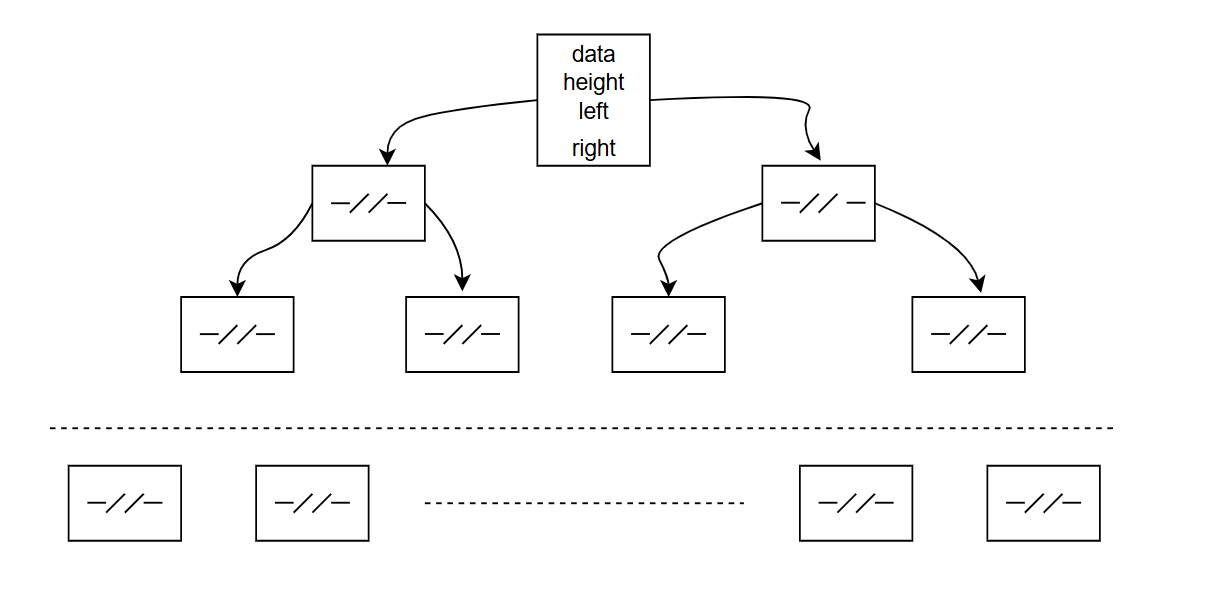
\includegraphics[width=1\textwidth]{vis_tree}
        \caption{Структура дерева}
    \end{figure}

    \subsection{Структура данных}

    Для хранения информации о материалах будет использоваться АВЛ-дерево, где ключом является код детали 
    \texttt{unit\_code}. Предполагается, что данные загружаются из \texttt{.csv} файла динамически.

    Ниже представлена реализация узла дерева:

    \begin{verbatim}
    typedef struct node {
        char unit_code[MAX_LEN_UNIT];     
        char material_code[MAX_LEN_MATERIAL];
        char measure[MAX_LEN_MEASURE];
        char production_id[MAX_LEN_PRODUCTION];
        char expected_consumption[MAX_LEN_E_CON];
        int height;                        
        struct node* left;
        struct node* right;
    } node;

    node* root = NULL;                     
    \end{verbatim}
    \begin{center}
        \vspace{-1.5em}
        \captionof{figure}{Структура узла АВЛ-дерева}
    \end{center}

    \subsection{Вспомогательные функции}

    Для работы с АВЛ-деревом необходимы следующие вспомогательные функции:

    \begin{verbatim}
    int height(node* x) {
        return x ? x->height : -1;
    }

    int difference_heights(node* x) {
        return x ? height(x->left) - height(x->right) : 0;
    }

    void update_height(node* x) {
        int h_left = height(x->left);
        int h_right = height(x->right);
        x->height = (h_left > h_right ? h_left : h_right) + 1;
    }
    \end{verbatim}
    \begin{center}
        \vspace{-1.5em}
        \captionof{figure}{Функции для работы с высотой узлов}
        \label{code:avl_utils}
    \end{center}

    \subsection{Балансировка дерева}

    Для поддержания сбалансированности АВЛ-дерева используются малые и большие повороты:

    \begin{verbatim}
    node* ll_rotation(node* x) {
        node* y = x->left;
        x->left = y->right;
        y->right = x;
        
        update_height(x);
        update_height(y);
        return y;
    }

    node* rr_rotation(node* x) {
        node* y = x->right;
        x->right = y->left;
        y->left = x;
        
        update_height(x);
        update_height(y);
        return y;
    }
    \end{verbatim}
    \begin{center}
        \vspace{-1.5em}
        \captionof{figure}{Функции малых поворотов}
    \end{center}

    \begin{figure}[H]
        \centering
        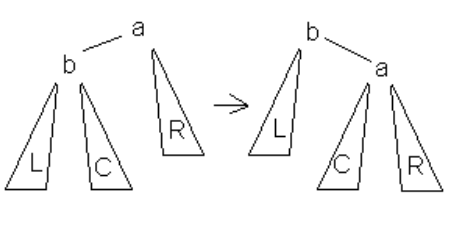
\includegraphics[width=0.7\textwidth]{rr}
        \caption{Схема малого правого поворота (LL-rotation)}
    \end{figure}

    \begin{figure}[H]
        \centering
        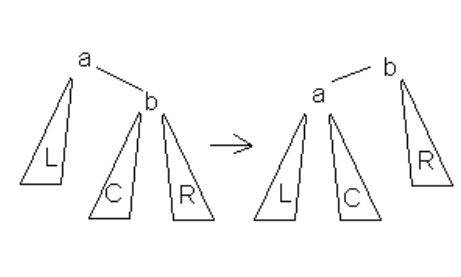
\includegraphics[width=0.7\textwidth]{ll}
        \caption{Схема малого левого поворота (RR-rotation)}
    \end{figure}

    \begin{verbatim}
    node* rl_rotation(node* x) {
        node* y = x->right;
        node* z = y->left;
        
        x->right = z->left;
        y->left = z->right;
        z->left = x;
        z->right = y;
        
        update_height(x);
        update_height(y);
        update_height(z);
        return z;
    }

    node* lr_rotation(node* x) {
        node* y = x->left;
        node* z = y->right;
        
        x->left = z->right;
        y->right = z->left;
        z->left = y;
        z->right = x;
        
        update_height(x);
        update_height(y);
        update_height(z);
        return z;
    }
    \end{verbatim}
    \begin{center}
        \vspace{-1.5em}
        \captionof{figure}{Функции больших поворотов}
    \end{center}

    \begin{figure}[H]
        \centering
        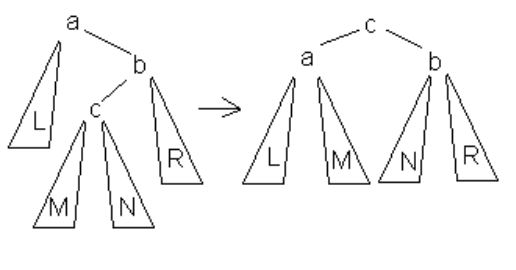
\includegraphics[width=0.8\textwidth]{rl}
        \caption{Схема большого левого поворота (RL-rotation)}
    \end{figure}

    \begin{figure}[H]
        \centering
        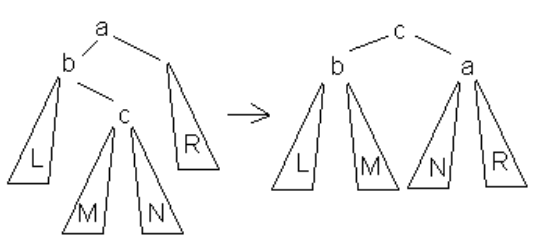
\includegraphics[width=0.8\textwidth]{lr}
        \caption{Схема большого правого поворота (LR-rotation)}
    \end{figure}

    \subsection{Операции с деревом}

    \textbf{Поиск элемента:}

    \begin{verbatim}
    node* find(node* x, const char* unit_code) {
        if(x == NULL)
            return NULL;
        
        int cmp = strcmp(unit_code, x->unit_code);
        
        if(cmp == 0)
            return x;
        
        if(cmp < 0)
            return find(x->left, unit_code);
        else
            return find(x->right, unit_code);
    }
    \end{verbatim}
    \begin{center}
        \vspace{-1.5em}
        \captionof{figure}{Функция поиска узла по коду детали}
    \end{center}

    \textbf{Вставка элемента:}

    \begin{verbatim}
    node* insert(node* x, node* new_node) {
        if (x == NULL) {
            return new_node;
        }
        
        int cmp = strcmp(new_node->unit_code, x->unit_code);
        
        if (cmp < 0) {
            x->left = insert(x->left, new_node);
        } else if (cmp > 0) {
            x->right = insert(x->right, new_node);
        } else {
            *x = *new_node;  
            free(new_node);
            return x;
        }
        
        update_height(x);
        int balance = difference_heights(x);
        
        if (balance > 1 && strcmp(new_node->unit_code,
         x->left->unit_code) < 0) {
            return ll_rotation(x);
        }
        if (balance < -1 && strcmp(new_node->unit_code,
         x->right->unit_code) > 0) {
            return rr_rotation(x);
        }
        if (balance > 1 && strcmp(new_node->unit_code,
         x->left->unit_code) > 0) {
            x->left = rr_rotation(x->left);
            return ll_rotation(x);
        }
        if (balance < -1 && strcmp(new_node->unit_code,
         x->right->unit_code) < 0) {
            x->right = ll_rotation(x->right);
            return rr_rotation(x);
        }
        return x;
    }
    \end{verbatim}
    \begin{center}
        \vspace{-1.5em}
        \captionof{figure}{Функция вставки узла в дерево}
    \end{center}

    \textbf{Удаление элемента:}

    \begin{verbatim}
    node* find_min(node* x) {
        while (x->left != NULL)
            x = x->left;
        return x;
    }

    node* delete(node* x, const char* unit_code) {
        if (x == NULL)
            return NULL;
        
        int cmp = strcmp(unit_code, x->unit_code);
        
        if (cmp < 0) {
            x->left = delete(x->left, unit_code);
        } else if (cmp > 0) {
            x->right = delete(x->right, unit_code);
        } else {
            if (x->left == NULL || x->right == NULL) {
                node* temp = x->left ? x->left : x->right;
                if (temp == NULL) {
                    free(x);
                    return NULL;
                } else {
                    *x = *temp;
                    free(temp);
                }
            } else {
                node* min_right = find_min(x->right);
                strcpy(x->unit_code, min_right->unit_code);
                strcpy(x->material_code, min_right->material_code);
                strcpy(x->measure, min_right->measure);
                strcpy(x->production_id, min_right->production_id);
                strcpy(x->expected_consumption, min_right->expected_consumption);
                x->height = min_right->height;
                x->right = delete(x->right, min_right->unit_code);
            }
        }
        
        if (x == NULL)
            return NULL;
        
        update_height(x);
        int balance = difference_heights(x);
        
        if (balance > 1 && difference_heights(x->left) >= 0) {
            return ll_rotation(x);
        }
        if (balance > 1 && difference_heights(x->left) < 0) {
            x->left = rr_rotation(x->left);
            return ll_rotation(x);
        }
        if (balance < -1 && difference_heights(x->right) <= 0) {
            return rr_rotation(x);
        }
        if (balance < -1 && difference_heights(x->right) > 0) {
            x->right = ll_rotation(x->right);
            return rr_rotation(x);
        }
        return x;
    }
    \end{verbatim}
    \begin{center}
        \vspace{-1.5em}
        \captionof{figure}{Функция удаления узла из дерева}
    \end{center}
    \clearpage
    \subsection{Оценка эффективности}

    Использование АВЛ-дерева вместо таблицы со статическим массивом даёт следующие преимущества:

    \begin{itemize}
        \item \textbf{Динамическое расширение:} отсутствие ограничения на максимальное количество записей $K$
        \item \textbf{Гарантированное время поиска:} $O(\log K)$ вместо ожидаемого $O(1)$ при хэшировании
        \item \textbf{Эффективная корректировка:} $O(\log K)$ против $O(K)$ при удалении сдвигом
        \item \textbf{Автоматическая упорядоченность:} данные всегда отсортированы по ключу
    \end{itemize}

    Недостатком является дополнительная память на хранение указателей и высоты узлов:
    \begin{itemize}
        \item Для $K$ узлов требуется дополнительно $K \cdot (2 \cdot 8 + 4)$ байт
        \item Временные затраты на балансировку при вставке и удалении
    \end{itemize}

    Таким образом, АВЛ-дерево является эффективной альтернативой для динамически изменяемых данных с частыми операциями поиска и корректировки.
    \clearpage
    \section*{Заключение}
    \refstepcounter{section}

    \begin{table}[H]
        \centering
        \small
        \renewcommand{\arraystretch}{1.8}
        \begin{tabular}{|>{\centering\arraybackslash}p{4cm}|>{\centering\arraybackslash}p{2.5cm}|>{\centering\arraybackslash}p{2.5cm}|>{\centering\arraybackslash}p{3cm}|>{\centering\arraybackslash}p{3cm}|}
            \hline
            & \textbf{Структура данных} & \textbf{Алгоритм поиска} & \textbf{Алгоритм упорядочивания} & \textbf{Корректировка} \\
            \hline
            \textbf{Исходный вариант} & Статический массив & Вычисление адреса & Пузырьком & Удаление сдвигом \\
            \cline{2-5}
            & $37K$ байт & $18L + 42$ & \(\displaystyle \frac{K(K-1)}{2}\) & $13 + 230(K-i-1)$ \\
            \hline
            \textbf{Альтернативный вариант} & АВЛ-дерево & Бинарный поиск & Не требуется & Удаление с балансировкой \\
            \cline{2-5}
            & $57K$ байт & $O(\log K)$ & \textbf{---} & $O(\log K)$ \\
            \hline
        \end{tabular}
        \caption{Сравнительный анализ исходного и альтернативного решения}
    \end{table}

    \vspace{-0.3cm}
    \begin{flushleft}
        \textit{Примечание: $K$ \textbf{—} количество записей, $L$ \textbf{—} длина кода детали, $i$ \textbf{—} индекс удаляемого элемента.}
    \end{flushleft}



\end{document}